\documentclass[11pt]{article}
% Adapted from an original template by Hlyni Arnórssyni,
% Reykjavik University, Iceland

% ------------------------------ PAGE SETTINGS ------------------------------
\usepackage{geometry}

\geometry{
    paper=a4paper,
    top=2.5cm,
    bottom=2.5cm,
    left=2.5cm,
    right=2.4cm,
    headheight=0.75cm,
    footskip=1.5cm,
    headsep=0.75cm
}

% ------------------------------ BASIC PACKAGES ------------------------------
\usepackage{blindtext}

% Character encoding
\usepackage[T1]{fontenc}
\usepackage[utf8]{inputenc}

% Mathematics
\usepackage{amsmath, amsfonts, amsthm, amssymb}
\usepackage{braket, nicefrac}

% SI units
\usepackage{siunitx}

% Lists / columns
\usepackage{enumitem, multicol}

% ------------------------------ FIGURES ------------------------------
\usepackage{graphicx}
\usepackage{float}
\usepackage{keystroke}
\usepackage{pgfplots}
\usepgfplotslibrary{units}
\pgfplotsset{compat=1.16}

% Search these locations automatically for figures
\graphicspath{{fig/}{graphics/}{Graphics/}{./}}

% ------------------------------ TABLES ------------------------------
\usepackage{tabularx}
\usepackage{array}
\usepackage[table]{xcolor}

% ------------------------------ TYPOGRAPHY ------------------------------
\usepackage{caption}
\usepackage{titlesec}
\usepackage{microtype}
\usepackage{csquotes}

% ------------------------------ COLORS ------------------------------
\definecolor{GWBlue}{HTML}{1E4E79}

% ------------------------------ SECTION STYLING ------------------------------
\titleformat{\section}
  {\Large\bfseries\color{GWBlue}}
  {\thesection.}
  {0.40em}
  {}

\titlespacing*{\section}
  {0pt}
  {0.70em}
  {0.28em}

% ------------------------------ CAPTION STYLING ------------------------------
\captionsetup{
    font=small,
    labelfont=bf,
    textfont=it,
    labelsep=period,
    skip=4pt
}

% ------------------------------ PARAGRAPH SPACING ------------------------------
\setlength{\parindent}{0pt}
\setlength{\parskip}{0.30em}

% ------------------------------ BIBLIOGRAPHY ------------------------------
\usepackage[
    backend=biber,
    style=authoryear,
    sorting=none,
    giveninits=true,
    maxbibnames=99,
    dashed=false
]{biblatex}

\addbibresource{references.bib}

\DeclareNameAlias{sortname}{family-given}
\DeclareNameAlias{default}{family-given}
\DeclareFieldFormat[article]{title}{#1}
\DeclareFieldFormat[misc]{title}{#1}
\renewbibmacro{in:}{}

\AtEveryBibitem{%
    \clearfield{doi}%
    \clearfield{urldate}%
}

\AtBeginBibliography{\small}
\setlength{\bibitemsep}{0.35em}

% ------------------------------ HYPERLINKS ------------------------------
\usepackage{hyperref}

\hypersetup{
    colorlinks=true,
    linkcolor=GWBlue,
    citecolor=GWBlue,
    urlcolor=GWBlue
}

\begin{document}

\begin{titlepage}
\centering
\thispagestyle{empty}

\vspace*{0.15in}


\includegraphics[
    width=0.5\textwidth
]{gwu_logo.pdf}

\vspace{0.28in}

{\large\bfseries Data Science Program\par}
{\large\bfseries Department of Data Science\par}
{\large DATS 6501 - Capstone Project - Fall 2026\par}

\vspace{0.38in}

{\Large\bfseries
Post-Training Analysis \& Novelty Detection Using\par}

\vspace{0.08in}

{\Large\bfseries
Neural Network Self-Organizing Maps (NNSOM)\par}

\vspace{0.34in}

{\large\bfseries
PHASE 1 REPORT\par}

\vspace{0.22in}

{\large\bfseries
Baseline Model Training \& Latent Feature Extraction\par}
\vspace{0.12in}
{\large\bfseries Fashion-MNIST\par}

\vspace{0.36in}

{\large\bfseries Capstone - Group 5\par}

\vspace{0.08in}

{\large\bfseries Fyrooz Anika Khan\par}
{\large\bfseries Nazish Atta\par}

\vspace{0.30in}

{\large The George Washington University\par}
{\large Washington, DC\par}

\vspace{0.30in}

{\large\itshape Supervised by\par}
{\large\itshape Dr. Amir Jafari\par}
{\large\itshape Associate Professor of Data Science\par}

\vspace*{\fill}

\end{titlepage}

\setcounter{page}{2}
\newcommand{\tbd}{\textbf{[TBD]}}

\section{Overview}

Phase 1 repeats the MNIST baseline on Fashion-MNIST \cite{xiao2017fashion}, a harder dataset of small grayscale pictures of clothing and shoes. The rule for the whole Fashion-MNIST study is to copy the MNIST design unchanged: the same split, the same LeNet-5 network and the same training recipe, \emph{not tuned} for the new data. So this phase answers one question: how well does the MNIST recipe do on a harder dataset, and does it give embeddings the SOM can work with?

\textbf{Summary of the results.}
\begin{itemize}[leftmargin=1.4em, itemsep=1pt]
  \item The network gets \textbf{90.90\%} of the test images right (95\% Wilson interval 90.33--91.43\%), against 99.18\% on MNIST. It makes 956 mistakes on 10,500 test images, about ten times as many as on MNIST.
  \item The 70,000 images are split evenly: every class has exactly 10\% of each split.
  \item The mistakes are not spread evenly. Most of them are between the four upper-body classes: \emph{T-shirt/top}, \emph{Pullover}, \emph{Coat} and \emph{Shirt}. \emph{Shirt} is the hardest class (F1 0.746).
  \item Trousers, sandals, bags and ankle boots are almost always right (F1 0.97--0.99).
  \item The 84-number \texttt{fc2} embeddings of every image are saved for Phase 2. With 876 mistakes on the validation images (against 92 on MNIST), Phase 2 has far more errors to study.
\end{itemize}

\subsection*{Where each item of the plan is covered}

{\small
\renewcommand{\arraystretch}{1.12}
\begin{tabularx}{\textwidth}{|>{\raggedright\arraybackslash}p{0.52\textwidth}|X|}
\hline
\textbf{What Phase 1 asks for} & \textbf{Where} \\ \hline
Load and preprocess the dataset; visualize class distributions & Section~\ref{sec:method}, Figures~\ref{fig:samples} and~\ref{fig:dist} \\ \hline
Data loaders with augmentation & Section~\ref{sec:method}: the proposal asks for augmentation for CIFAR only; none is used here, as on MNIST \\ \hline
Evaluation metrics: accuracy, per-class F1, confusion matrix & Tables~\ref{tab:results} and~\ref{tab:perclass}, Figure~\ref{fig:cm} \\ \hline
Train a standard CNN (LeNet-5); record train, validation and test metrics & Figure~\ref{fig:curves}, Table~\ref{tab:results} \\ \hline
Choose the feature layer; save embeddings for all splits & Section~\ref{sec:latent} \\ \hline
\end{tabularx}}

\section{Key terms in plain words}

{\small
\renewcommand{\arraystretch}{1.12}
\begin{tabularx}{\textwidth}{|>{\raggedright\arraybackslash}p{0.24\textwidth}|X|}
\hline
\textbf{Term} & \textbf{What it means} \\ \hline
Training / validation / test images & Training images teach the network. Validation images are used to pick the best epoch. Test images are kept aside and used once at the end, like an exam. \\ \hline
Stratified split & Every class has the same share in each of the three parts. \\ \hline
LeNet-5 & A small convolutional network (CNN) first built for handwritten digits \cite{lecun1998gradient}. \\ \hline
Epoch & One pass of the network over all training images. \\ \hline
Accuracy, F1 & Accuracy is the share of images the network gets right. F1 combines how often a predicted class is right (precision) and how many images of a class are found (recall). Macro-F1 is the average over the 10 classes. \\ \hline
Wilson interval & A 95\% range for the true accuracy, given that only 10,500 test images were used. \\ \hline
Confusion matrix & A table of true class against predicted class; the diagonal holds the correct answers. \\ \hline
Embedding (\texttt{fc2}) & The 84 numbers the network computes for an image just before it gives its answer. Phase 2 trains the SOM on these numbers. \\ \hline
\end{tabularx}}

\section{Related Work}

LeCun et al.~\cite{lecun1998gradient} showed that convolutional networks learn useful features for handwritten digits; we use their LeNet-5 as a fixed source of features, not as a new classifier. Xiao et al.~\cite{xiao2017fashion} built Fashion-MNIST as a drop-in replacement for MNIST: the same image size, number of classes and split sizes, but with clothing, which is harder to tell apart. We use it for exactly that reason. It lets the whole MNIST pipeline run without changes, and it gives many more network mistakes for the SOM to study. The SOM and novelty-detection work that this baseline feeds into is described in the MNIST Phase 1 report and in the later phases \cite{kohonen1990som,jafari_nnsom}.

\section{Method}\label{sec:method}

\begin{table}[H]
\centering
\renewcommand{\arraystretch}{1.10}
\begin{tabular}{|p{0.36\textwidth}|p{0.54\textwidth}|}
\hline
\textbf{Item} & \textbf{Phase 1 setup (same as MNIST)} \\ \hline
Dataset & Fashion-MNIST: 60,000 + 10,000 grayscale images ($28\times28$) joined into 70,000, 10 classes \\ \hline
Classes (0--9) & T-shirt/top, Trouser, Pullover, Dress, Coat, Sandal, Shirt, Sneaker, Bag, Ankle boot \\ \hline
Split & Stratified 70/15/15, seed 42: 49,000 train / 10,500 validation / 10,500 test (4,900 / 1,050 / 1,050 per class) \\ \hline
Preprocessing & Pixel values divided by 255; nothing else, no augmentation \\ \hline
Model & LeNet-5, MNIST recipe: 20 epochs, Adam (learning rate 0.001, weight decay 0.0001), learning rate $\times0.1$ every 10 epochs, batch 64, seed 42 \\ \hline
Checkpoint & Epoch with the best validation accuracy \\ \hline
Feature layer & \texttt{fc2}, 84 numbers, saved for all three splits with sample IDs, labels, predictions and confidence \\ \hline
\end{tabular}
\caption{Phase 1 setup. Run ID \texttt{lenet5\_fashion\_mnist\_s42}.}
\end{table}

\begin{figure}[H]
\centering
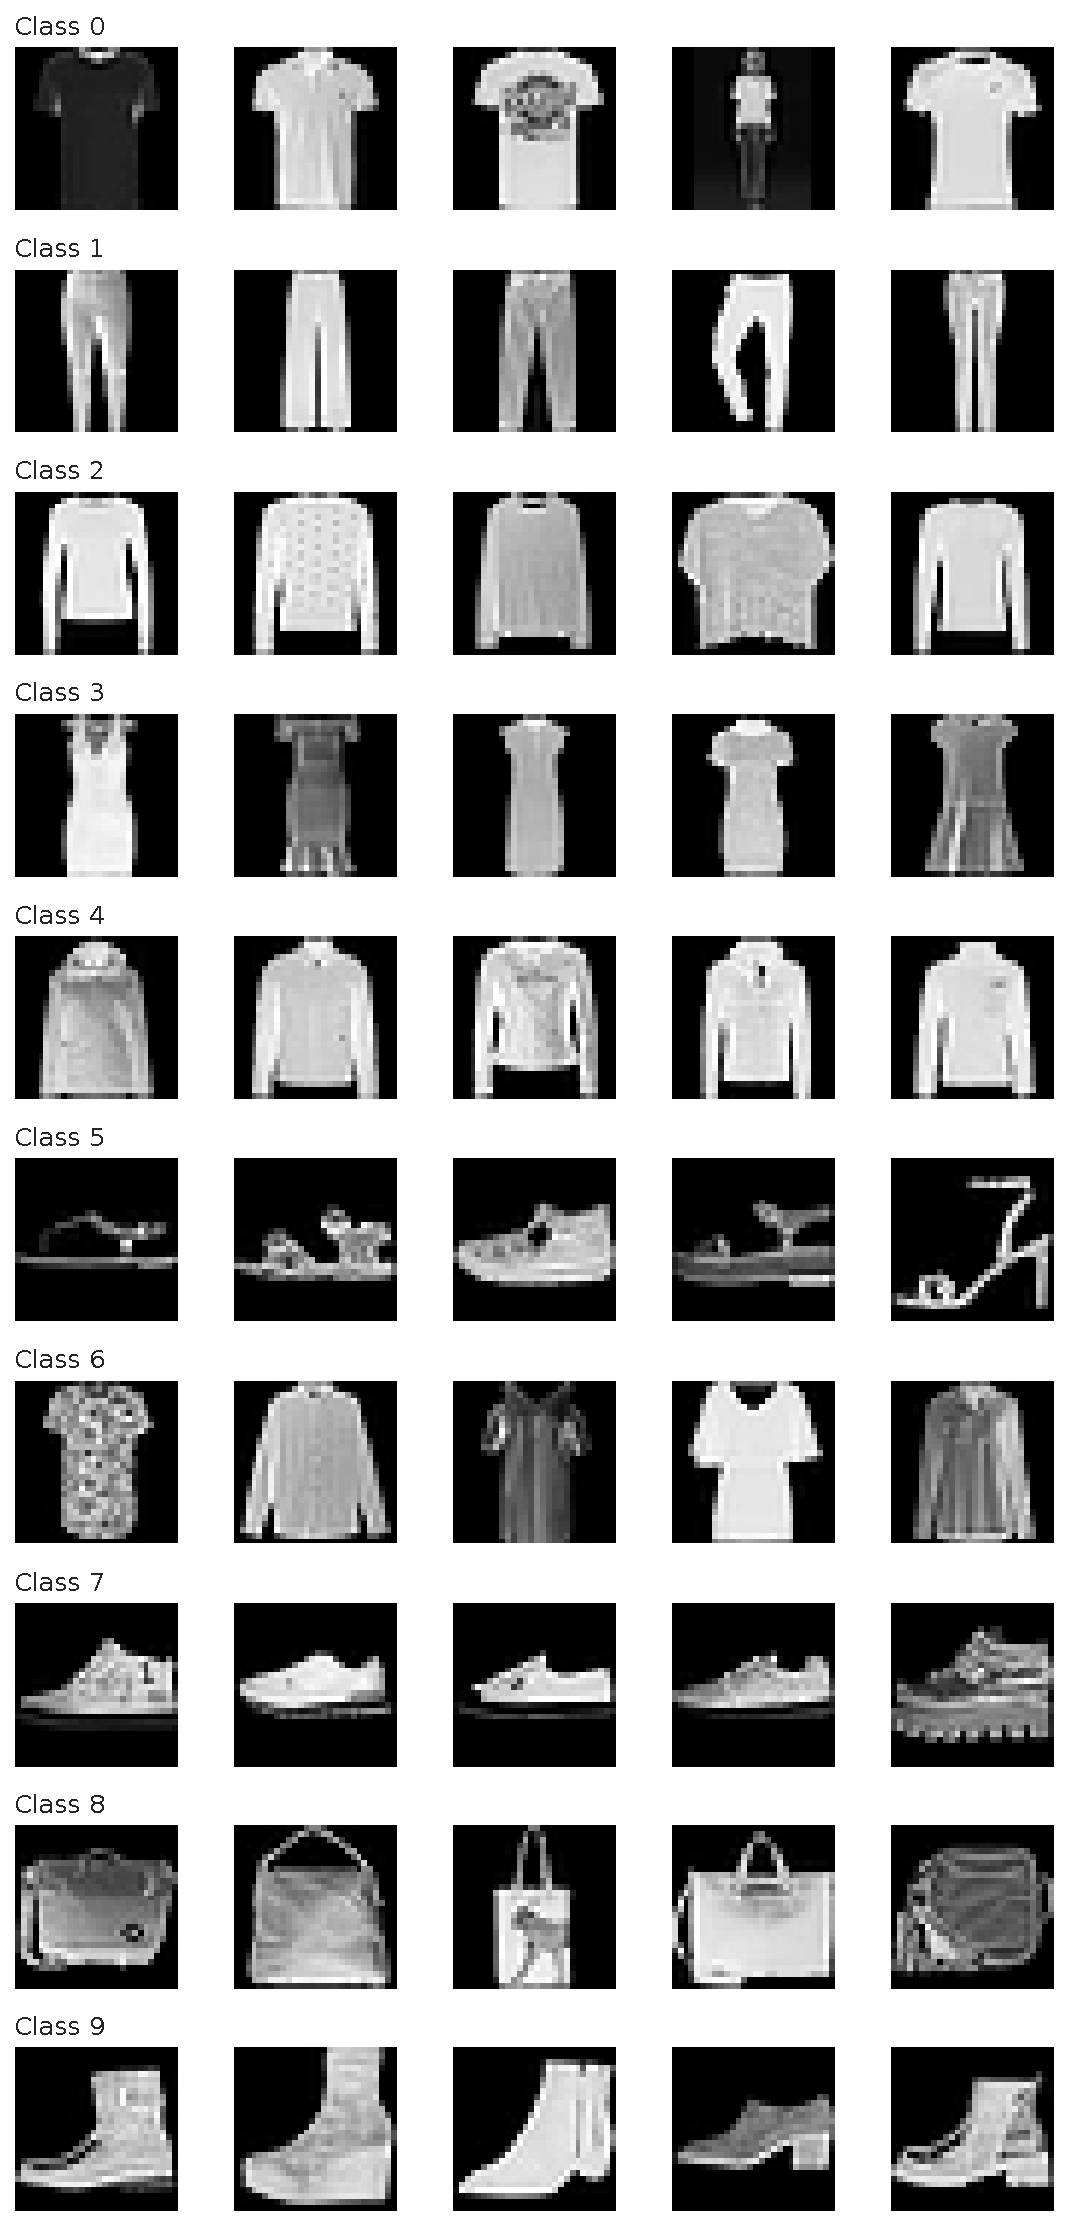
\includegraphics[width=0.62\textwidth,keepaspectratio]{fig/data_pipeline/sample_images.pdf}
\caption{Five training images of each class (0: T-shirt/top, 1: Trouser, 2: Pullover, 3: Dress, 4: Coat, 5: Sandal, 6: Shirt, 7: Sneaker, 8: Bag, 9: Ankle boot).}
\label{fig:samples}
\end{figure}

\textbf{Class distributions (Figure~\ref{fig:dist}).} The stratified split gives every class exactly the same share in every part: 4,900 training, 1,050 validation and 1,050 test images per class (10\% each). So no class is over- or under-represented, and accuracy is a fair summary on its own.

\begin{figure}[H]
\centering
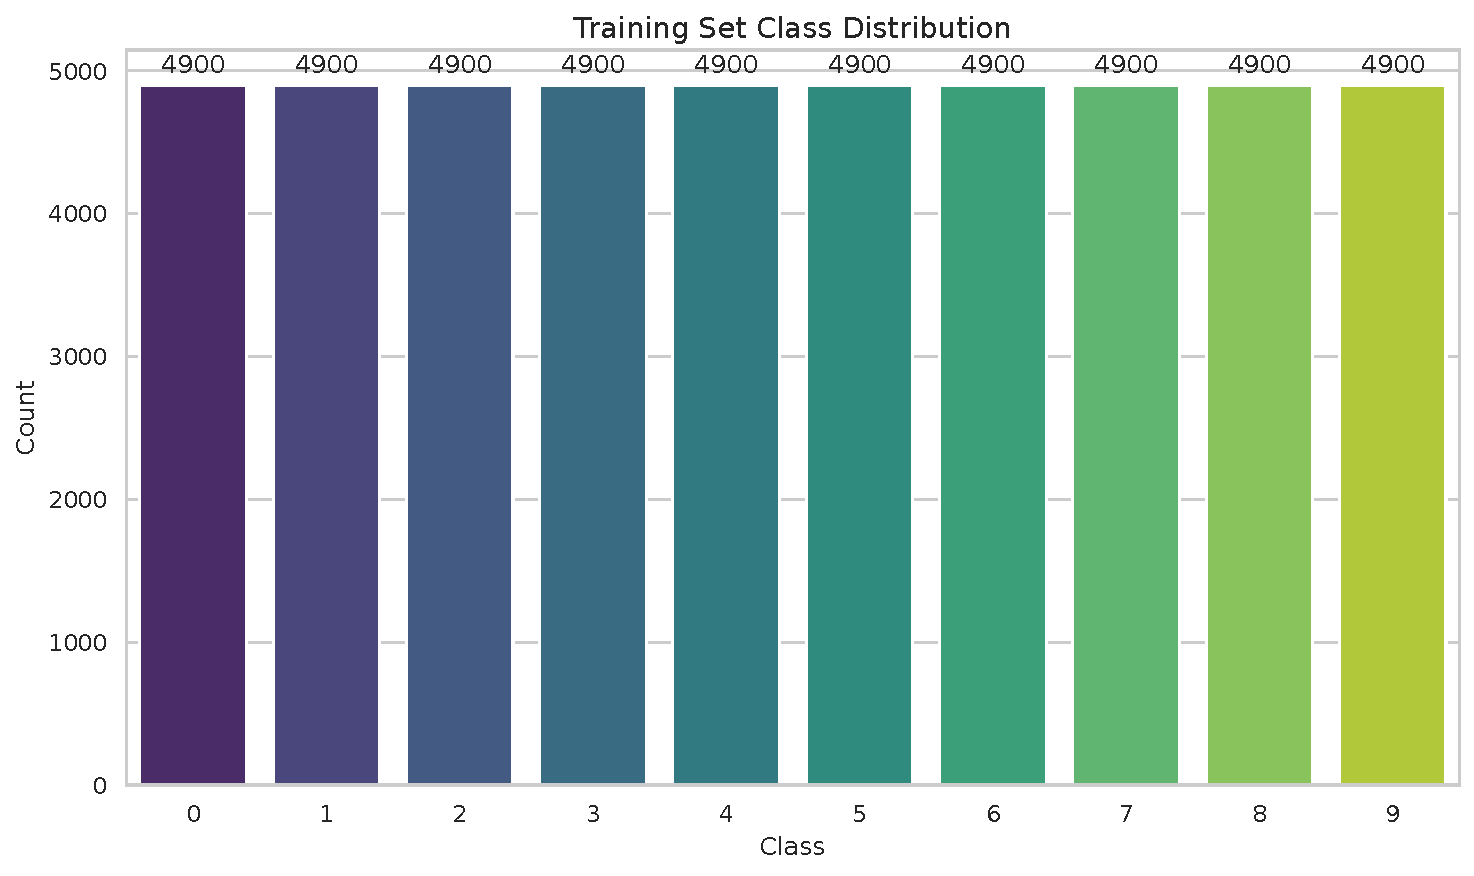
\includegraphics[width=0.32\textwidth,keepaspectratio]{fig/data_pipeline/train_dist.pdf}\hfill
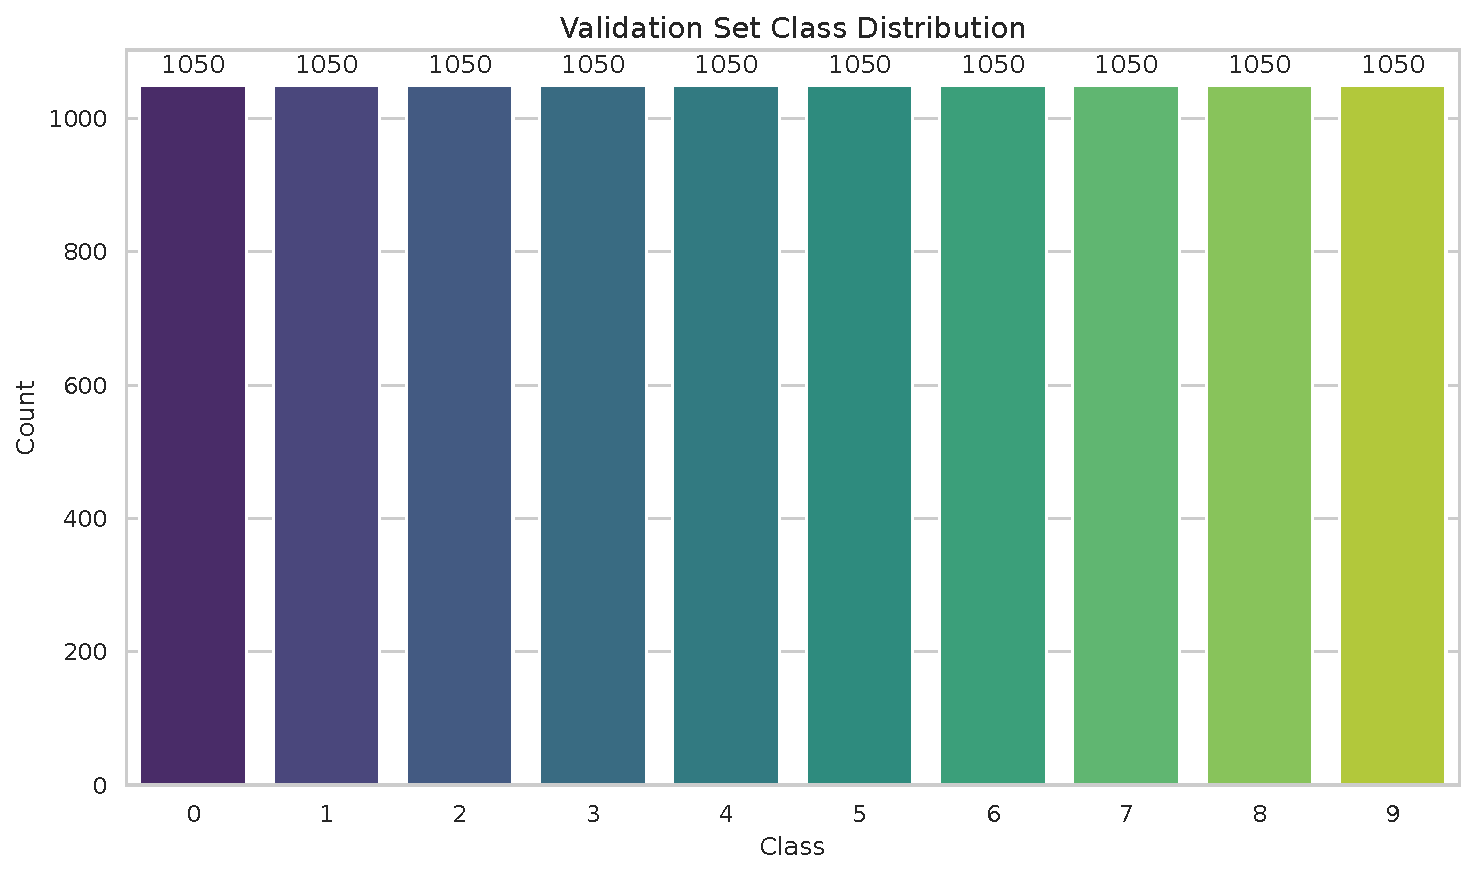
\includegraphics[width=0.32\textwidth,keepaspectratio]{fig/data_pipeline/val_dist.pdf}\hfill
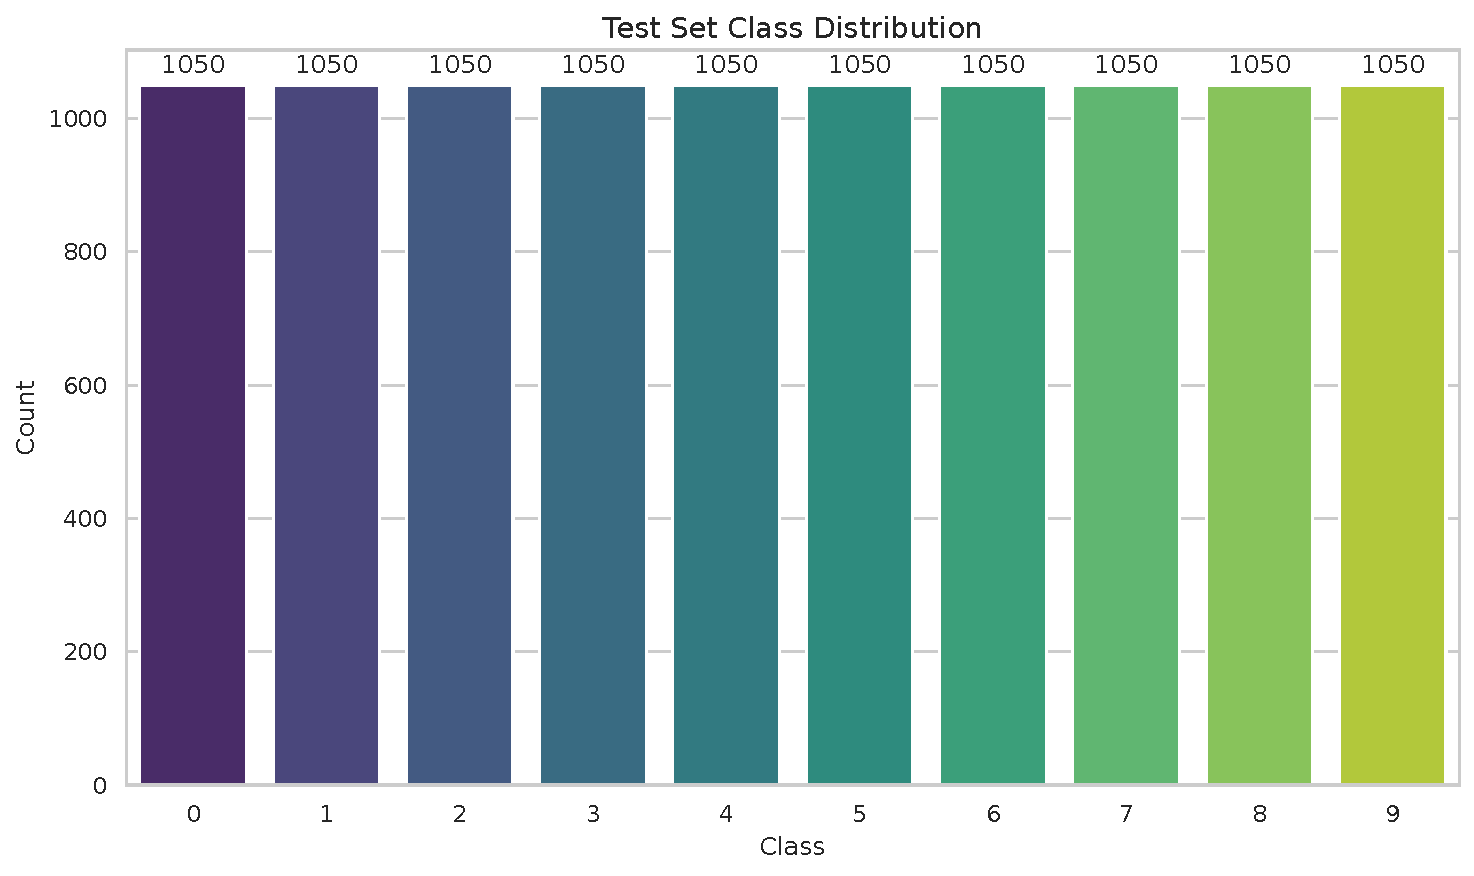
\includegraphics[width=0.32\textwidth,keepaspectratio]{fig/data_pipeline/test_dist.pdf}
\caption{Number of images per class in the training (left), validation (middle) and test (right) splits.}
\label{fig:dist}
\end{figure}

\section{Results}

\textbf{Training (Figure~\ref{fig:curves}).} Validation accuracy rises quickly to about 88\% by epoch 5, climbs again when the learning rate drops at epoch 10, and peaks at \textbf{91.66\%} in epoch 16, which is the checkpoint kept. At that checkpoint the network gets 93.24\% of the training images right (3,311 mistakes) against 91.66\% of the validation images (876 mistakes), so it fits the training images only a little better than new ones; it is not badly over-fitted.

\begin{figure}[H]
\centering
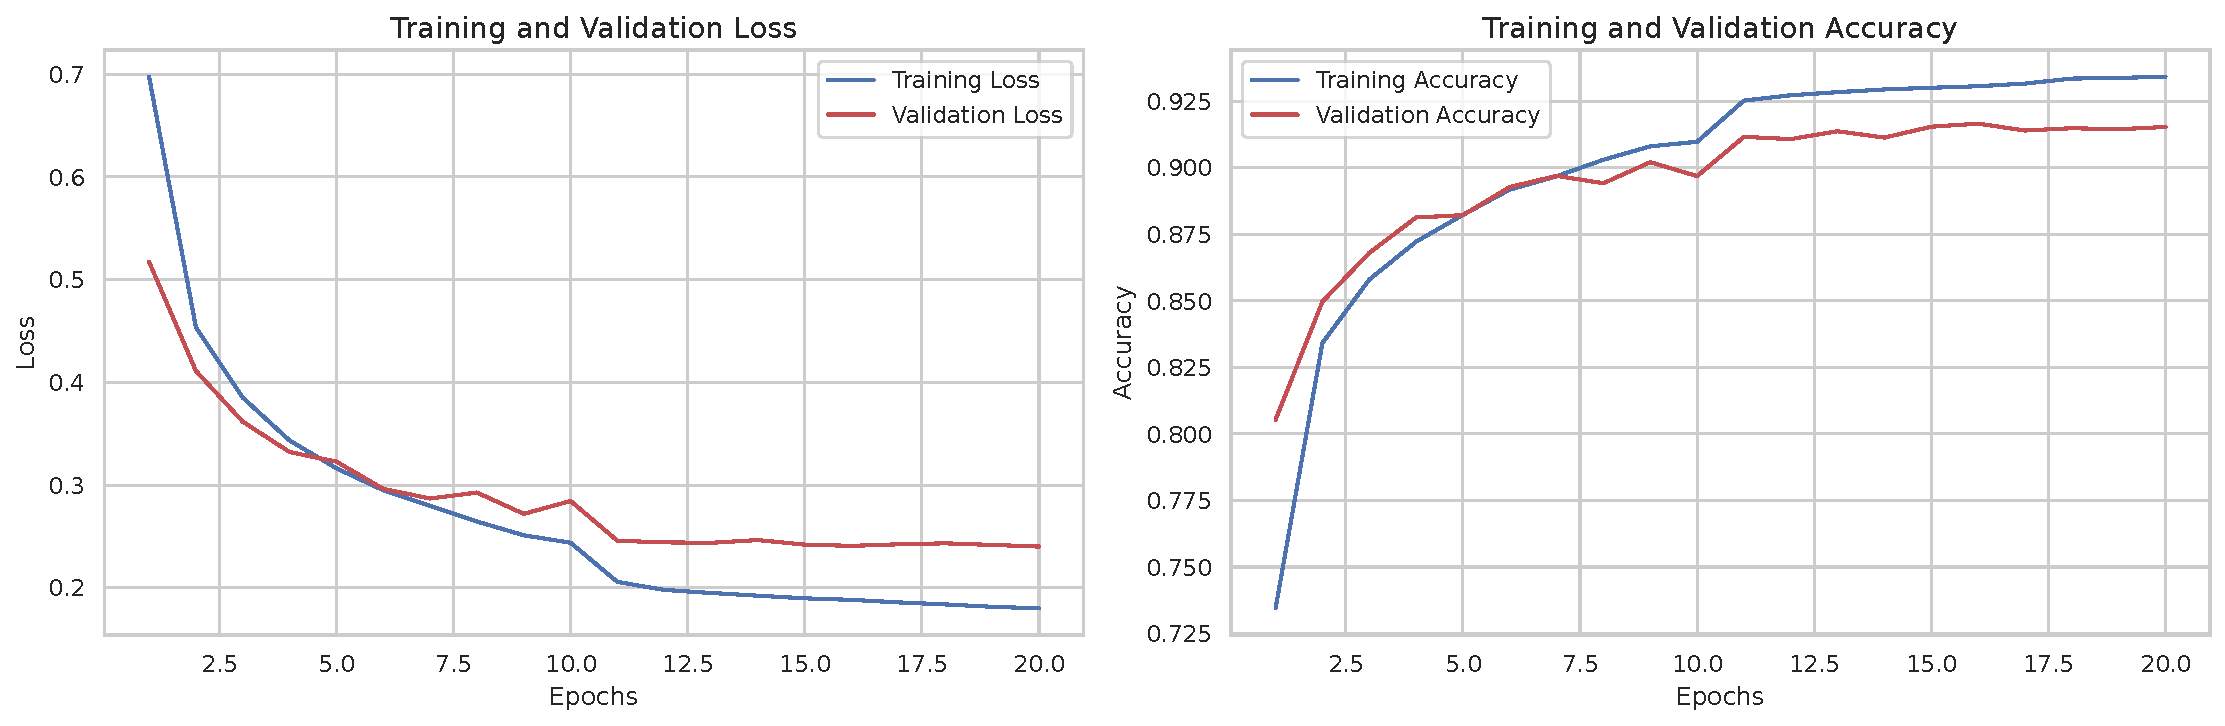
\includegraphics[width=0.92\textwidth,keepaspectratio]{fig/cnn_baseline/training_curves.pdf}
\caption{Training and validation loss (left) and accuracy (right) over the 20 epochs.}
\label{fig:curves}
\end{figure}

\begin{table}[H]
\centering
\renewcommand{\arraystretch}{1.10}
\begin{tabular}{|p{0.36\textwidth}|p{0.27\textwidth}|p{0.27\textwidth}|}
\hline
\textbf{Measure} & \textbf{Fashion-MNIST} & \textbf{MNIST (for reference)} \\ \hline
Test accuracy & 90.90\% (9,544 / 10,500) & 99.18\% (10,414 / 10,500) \\ \hline
95\% Wilson interval & 90.33--91.43\% & 98.99--99.34\% \\ \hline
Macro-F1 & 0.9089 & 0.9918 \\ \hline
Test mistakes & 956 (9.10\%) & 86 (0.82\%) \\ \hline
Validation accuracy (best epoch) & 91.66\% (876 mistakes) & 99.12\% (92 mistakes) \\ \hline
Training accuracy & 93.24\% & -- \\ \hline
\end{tabular}
\caption{Phase 1 results. The test split was evaluated once, at the end of training.}
\label{tab:results}
\end{table}

\begin{table}[H]
\centering
\renewcommand{\arraystretch}{1.08}
\small
\begin{tabular}{|l|c|c|c|}
\hline
\textbf{Class} & \textbf{Precision} & \textbf{Recall} & \textbf{F1} \\ \hline
0 T-shirt/top & 0.864 & 0.868 & 0.866 \\ \hline
1 Trouser & 0.992 & 0.981 & 0.987 \\ \hline
2 Pullover & 0.879 & 0.825 & 0.851 \\ \hline
3 Dress & 0.906 & 0.934 & 0.920 \\ \hline
4 Coat & 0.818 & 0.862 & 0.840 \\ \hline
5 Sandal & 0.982 & 0.972 & 0.977 \\ \hline
6 Shirt & 0.753 & 0.739 & \textbf{0.746} \\ \hline
7 Sneaker & 0.948 & 0.968 & 0.958 \\ \hline
8 Bag & 0.976 & 0.979 & 0.978 \\ \hline
9 Ankle boot & 0.974 & 0.962 & 0.968 \\ \hline
\end{tabular}
\caption{Test results per class (1,050 test images each).}
\label{tab:perclass}
\end{table}

\textbf{Where the mistakes are (Figure~\ref{fig:cm}).} The largest confusions on the test images are Shirt called T-shirt/top (110), T-shirt/top called Shirt (105), Pullover called Coat (90), Shirt called Coat (79), and Pullover or Coat called Shirt (62 each). All of them are between upper-body garments, which look alike at $28\times28$ pixels. Mistakes among T-shirt/top, Pullover, Coat and Shirt make up 638 of the 956 test mistakes (67\%). The footwear classes are sometimes mixed up with each other (for example, Ankle boot called Sneaker, 32), but almost never with anything else: of the 103 footwear images the network gets wrong, only 6 are called something other than footwear, and only 5 non-footwear images are called footwear. So the mistakes come from a few groups of similar classes, which is what Phase 2 tests on the SOM.

\begin{figure}[H]
\centering
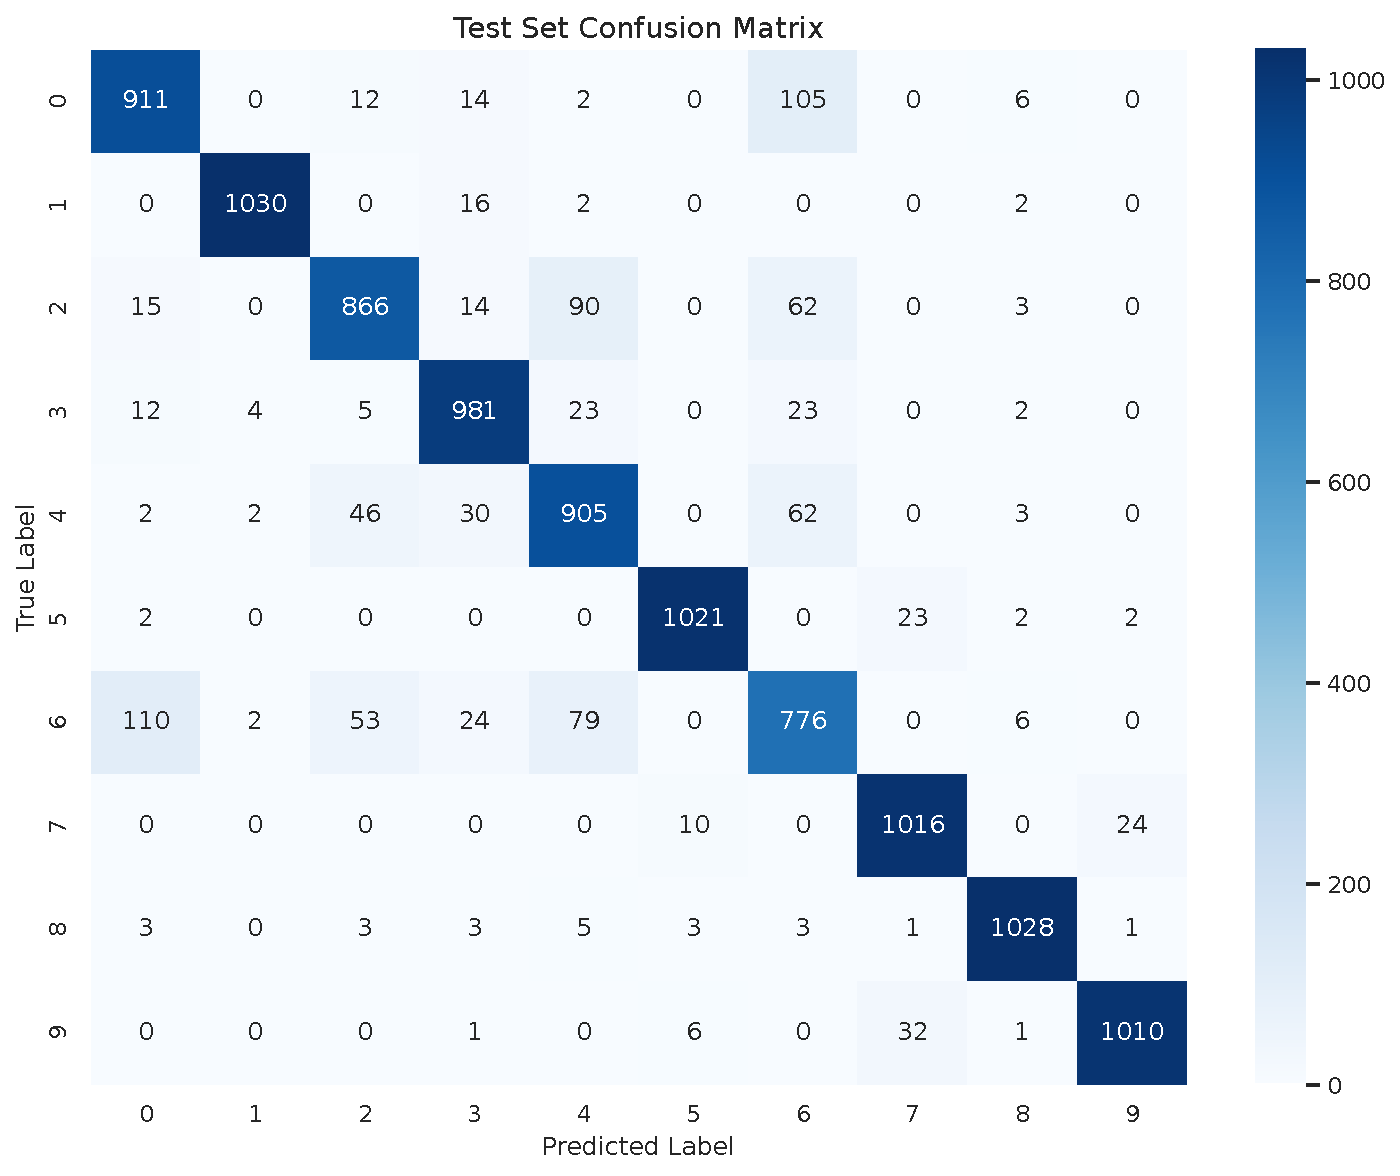
\includegraphics[width=0.66\textwidth,keepaspectratio]{fig/cnn_baseline/confusion_matrix.pdf}
\caption{Test confusion matrix (rows: true class, columns: predicted class; class numbers as in Figure~\ref{fig:samples}).}
\label{fig:cm}
\end{figure}

\section{Latent Feature Representation}\label{sec:latent}

For every image in the three splits, the 84 numbers of the \texttt{fc2} layer were saved, together with its sample ID, true class, predicted class, confidence and whether it was right. The saved files were checked when written: every value is finite, every sample ID is unique, and the counts match the split (49,000 / 10,500 / 10,500). Each file is fingerprinted with SHA-256 so later phases can check they use the same embeddings. The network is less sure of its answers than on MNIST: on validation images its mean confidence is 0.94 when it is right and 0.69 when it is wrong, against 0.997 and 0.833 on MNIST. This gap matters for the confidence-based baselines in Phases 2 and 3.

The MNIST Phase 1 report also showed a 2D PCA view of the embeddings and a page of misclassified test images. They are not part of the Phase 1 plan in the project proposal and no pipeline step produces them, so they are not repeated here. Phase 2 gives a fuller picture of the same embeddings (the SOM maps) and shows misclassified images from the error hotspots.

\section{Leakage Control}

\begin{itemize}
  \item The 70,000 images were split once, with a stratified split and a fixed seed (42), into training, validation and test parts. Every image keeps a fixed sample ID, so the parts never overlap.
  \item Pixels were only divided by 255. No statistic was computed from the data, and no augmentation was used.
  \item The network was trained on the training split only. The epoch was chosen by validation accuracy. All training settings were copied from MNIST and written down in the Fashion-MNIST protocol before any Fashion-MNIST data was loaded; nothing was tuned on Fashion-MNIST.
  \item The test split was evaluated once, after training, for the numbers above. By the protocol it is used once more, in the final test of Phase 4, and no setting is chosen from either use.
  \item Test embeddings are saved for completeness; Phase 2 uses the training and validation embeddings only.
  \item The run records the SHA-256 of its configuration, checkpoint and embedding files, and a finished run is never overwritten.
\end{itemize}

\section{Limitations}

\begin{itemize}[leftmargin=1.4em, itemsep=1pt]
  \item The network is deliberately not tuned for Fashion-MNIST, so 90.9\% describes the MNIST recipe on Fashion-MNIST, not the best a small CNN can reach on this data.
  \item One network with one seed; how much the accuracy varies between seeds is measured only in Phase 4.
\end{itemize}

\section{Conclusion and Transition to SOM Training}

The MNIST pipeline runs on Fashion-MNIST without changes and gives a baseline of 90.90\% test accuracy. Its mistakes gather between the upper-body garment classes, and the validation split holds 876 of them, about ten times as many as on MNIST. In Phase 2 the same 15$\times$15 SOM recipe \cite{jafari_nnsom} is trained on the 49,000 training embeddings to see whether these mistakes also gather in a few regions of the map.

\clearpage
\printbibliography[title={References}]

\end{document}
